\chapter{Introdução}

\section{Justificativa}

\section{Objetivo}

\subsection{ Objetivo Geral}

\subsection{Objetivos Específicos}


\section{Organização}
O presente trabalho está organizado da seguinte forma:





% Introduzir Figura
%\begin{figure}
%	   \centering
%	   		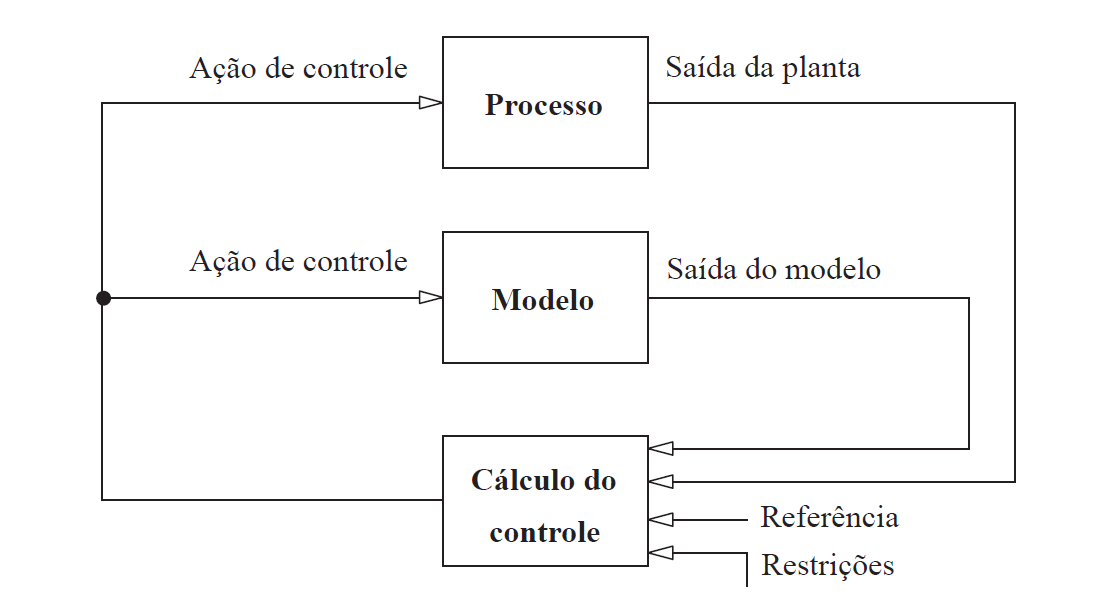
\includegraphics[scale=0.35]{figs/MPCbase.PNG} 
%	   \caption{Algoritmo MPC}
%	   \label{label para referencia cruzada Figura}
%\end{figure}


% Lista de Item

%\begin{itemize}
%	\item item 1
%	\item item 2
%	\item item 3
%\end{itemize}

% Equação
%\begin{equation}
%	\label{label para referencia cruzada %equacoes} 
%	y(t)=\sum_{i=1}^{\infty}h_i\Delta u(t-i)
%\end{equation}

% Equação em linha 
%$\hat{y}(t+k\mid t)= \sum^\infty_{i=1} g_i %\Delta u(t+k-i\mid t)$

% Citação -  Criei o arquivo de bibliografia usando o jabref

%\cite{Camacho2007} 

% Referencia Cruzada de Figura
%\ref{label para referencia cruzada Figura}

% Referencia Cruzada de Equação
%\ref{label para referencia cruzada equacoes}


% Tabelas

%\begin{table}[h]
%\begin{center}
%     \caption{Índices 1 para casos factíveis}
%     \begin{tabular}{| l | l | l | l |}
%     \hline Índice & LP Petro & LP 2 & %Diferença\\ 
%     \hline $SES_y$& 60.5406 & 60.5492 & %-0.0087\\
%     \hline $SES_u$& 1166.1464 & 1166.1464 & 2.36*$10^{-9}$ \\
%     \hline
 
%    \end{tabular}
%\label{table:indices1}
%\end{center}
%\end{table}